%%
%% Start line numbering here if you want
%%
% !TEX root = jetjtPaperPreview.tex
\linenumbers

%% main text
\section{Introduction}
\label{sec:introduction}
Jets are collimated sprays of hadrons originating from the fragmentation of hard partons produced in high-energy particle collisions. Studying the jet fragmentation can give insight into QCD phenomena, such as angular ordering~\cite{basicsofpqcd} and hadronization. In this study the fragmentation of partons is studied using the jet fragmentation transverse momentum, $\jt{}$, which is the perpendicular component of the momentum with respect to the momentum vector of the initial hard parton.

Recently $\jt{}$ with two-particle correlations was studied at ALICE~\cite{ALICEjt}. Previously, $\jt{}$ has been studied using two-particle correlations by the CCOR collaboration at ISR with $\pp$ collisions at center-of-mass energy $\sqrtS = 31,\;45$ and $63~\mathrm{GeV}$~\cite{firstjtmeasurement} and the PHENIX collaboration at RHIC with $\pp$ collisions at $\sqrtSE[GeV]{200}$~\cite{PHENIXjets} and d--Au collisions at center-of-mass energy per nucleon pair $\sqrtSnnE[GeV]{200}$~\cite{phenixJtPAu}. Jet measurements to study $\jt{}$ have been done by the CDF collaboration at the Tevatron with $\ppbar$ collisions at $\sqrtSE{1.96}$~\cite{cdfpaper} and the ATLAS collaboration at the LHC with $\PbPb$ collisions at $\sqrtSnnE{2.76}$~\cite{atlaksenJetit}.

Jet production in QCD can be thought of as two separate stages~\cite{eventGenerators}. After being produced in the hard scattering, partons reduce their high virtuality through emitting gluons. Since the transverse momentum scale ($Q^{2}$) is large during the showering, perturbative QCD calculations can be applied. When $Q^{2}$ becomes of the order of $\Lambda_{\mathrm{QCD}}$, partons hadronize into final-state particles through a non-perturbative process. 

In practice these two stages happen at least in part simultaneously. %{\color{red} [Showering time vs hadronization time ]}
Thus it is not a priori clear that the effect of these can be separated. However, two distinct components were identified in ALICE when studying $\jt{}$ with two-particle correlations~\cite{ALICEjt}.The goal of this study is to see if similar identification of components is possible in a full jet reconstruction based study. 

As non-perturbative processes these are hard to calculate from first principles. Instead Monte Carlo generators such as \textsc{Pythia}~\cite{introPythia81} and Herwig~\cite{Herwig7releaseNote} are used to produce a theoretical background. One approach based on perturbative QCD (pQCD) is the Next-to-Modified Leading Log Approximation (NMLLA)~\cite{nmlla}. This approach implements local parton hadron duality (LPHD) instead of any more sophisticated hadronization model.

These two MC generators handle both the showering process and hadronization differently. Pythia uses the Lund string model~\cite{lundString} to perform the hadronization stage. Herwig uses a cluster model for the hadronization. Pythia 6 has $\pt{}$ ordered showers while Pythia 8 has rapidity ordered showers. Herwig simulates parton showers using the coherent branching algorithm of~\cite{Gieseke:2003rz}. This algorithm has angular ordering as a central feature. In \textsc{Pythia} 8 angular ordering is built in, while in \textsc{Pythia} 6 it can be turned on or off.

In this paper, the $\jt{}$ distributions are studied by reconstructing the jets with jet algorithms~\cite{antikt} in $\sqrtSnnE{5.02}$ $\pPb$ collisions. The advantage of jet reconstruction is that it should give a better estimate of the initial hadron momentum when compared to using two-particle correlations. Additionally the results are not smeared by the splitting of the leading hadron as was the case in the correlation study. The disadvantage is that the jet reconstruction limits the study to a small cone around the jet axis. Additionally the kinematics of produced jets are different. In dihadron analysis, the results are done in $\pt{trigger}$ bins, which favours harder jets (leading track carries a large fraction of the momentum). When looking at $\pt{jet}$ bins softer jets are favoured.

The presence of a heavy nucleus as in p--A collisions might alter the fragmentation process. One possible mechanism for this is initial or final-state scattering of partons inside the nucleus. However in dihadron analysis it was found that there is no difference in $\jt{}$ between $\pp$ and $\pPb$ collisions~\cite{ALICEjt}.

This paper is structured as follows. The event and track selection together with the used data samples are described in Sec.~\ref{sec:experimentaldetails}. The analysis details are discussed in Sec.~\ref{sec:methods}, followed by the systematic uncertainty analysis in Sec.~\ref{sec:systematicerrors}. The obtained results are shown in Sec.~\ref{sec:results} and the observations are summarized in Sec.~\ref{sec:conclusions}.

 

%Jets are collimated sprays of hadrons originating from the fragmentation of hard partons produced in high-energy particle collisions. Studying the jet fragmentation can provide information about QCD color coherence phenomena, such as angular ordering~\cite{basicsofpqcd}, and constrain hadronization models. The transverse fragmentation of partons is often studied using the jet fragmentation transverse momentum, $\jt{}$, the momentum component of particles produced in the fragmentation perpendicular to the momentum vector of the hard parton initiating the fragmentation. Previously, $\jt{}$ has been studied using two-particle correlations by the CCOR collaboration at ISR with $\pp$ collisions at center-of-mass energy $\sqrtS = 31,\;45$ and $63~\mathrm{GeV}$~\cite{firstjtmeasurement} and the PHENIX collaboration at RHIC with $\pp$ collisions at $\sqrtSE[GeV]{200}$~\cite{PHENIXjets} and d--Au collisions at center-of-mass energy per nucleon pair $\sqrtSnnE[GeV]{200}$~\cite{phenixJtPAu}. Jet measurements to study $\jt{}$ have been done by the CDF collaboration at the Tevatron with $\ppbar$ collisions at $\sqrtSE{1.96}$~\cite{cdfpaper} and the ATLAS collaboration at the LHC with $\PbPb$ collisions at $\sqrtSnnE{2.76}$~\cite{atlaksenJetit}.
%
%Jet fragmentation in QCD consists of two different steps~\cite{eventGenerators}. After the hard scattering, partons go through a QCD induced showering step, where gluons are emitted and the high virtuality  of the parton is reduced. Since the transverse momentum scale ($Q^{2}$) is large during the showering, perturbative QCD calculations can be applied. When $Q^{2}$ becomes of the order of $\Lambda_{\mathrm{QCD}}$, partons hadronize into final-state particles through a non-perturbative process. Two distinct components, related to the showering and hadronization phases, can be identified from the measured $\jt{}$~distributions.
%
%The presence of a heavy nucleus as in p--A collisions might alter the fragmentation process. One possible mechanism for this is initial or final-state scattering of partons inside the nucleus. This is expected to lead to a broadening of jets, since the scattered partons are likely to deviate from their original direction~\cite{jetBroadeningPpb1}. Also the nuclear parton distribution functions can change the relative contributions of quarks and gluons compared to free nucleons, for example via gluon saturation and shadowing effects~\cite{introCgc,eps09}. Understanding the implications of these cold nuclear matter effects will provide an important baseline for similar measurements in heavy-ion collisions.
%
%In this paper, the $\jt{}$ distributions are studied using two-particle correlations measured by the ALICE detector in $\sqrtSE{7}$ $\pp$ and $\sqrtSnnE{5.02}$ $\pPb$ collisions. The correlation approach is chosen as opposed to full jet reconstruction based on the discussion in Ref.~\cite{thorstenBiasProceedings,Renk:2011wp}, where it is argued that two-particle correlations are more sensitive to the soft and non-perturtabive parts of the jet fragmentation. This is important for the separation of the two $\jt{}$ components and in searching for cold nuclear matter effects.
%

\section{Experimental setup and data samples}
\label{sec:experimentaldetails}
The $\sqrtSnnE{5.02}$ $\pPb$ ($1.3 \cdot 10^{8}$ events, $\mathcal{L}_{\mathrm{int}} = \unit{620}{nb^{-1}}$) collisions were recorded in 2013 by the ALICE detector~\cite{aliceDetector}. The details of the performance of the ALICE detector during LHC Run~1 (2009-2013) are presented in Ref.~\cite{alicePerformance}.

The analysis uses charged tracks that are reconstructed with the Inner Tracking System (ITS)~\cite{aliceITS} and the Time Projection Chamber (TPC)~\cite{aliceTPC}. These detectors are located inside the large solenoidal magnet, that provides a homogeneous magnetic field of $\unit{0.5}{T}$. Tracks within a pseudorapidity range $|\eta| < 0.9$ over the full azimuth can be reconstructed. The ITS is made up of the innermost Silicon Pixel Detector (SPD), the Silicon Drift Detector (SDD) and the outermost Silicon Strip Detector (SSD). Each of these consists of two layers. The TPC is a cylinder filled with gas. Gas is ionised along the path of charged particles. Liberated electrons drift towards the end plates of the cylinder where they are detected. Combining the information from the ITS and the TPC provides a resolution ranging from $1$ to $10\,\%$ for charged particles with momenta from $0.15$ to $100~\GeVc$. For tracks without the ITS information, the momentum resolution is comparable to that of ITS+TPC tracks below transverse momentum $\pt{} = 10~\GeVc$, but for higher momenta the resolution reaches $20\,\%$ at $\pt{} = 50~\GeVc$~\cite{alicePerformance,aliceBackgroundFluctuation}. 

Neutral particles used in jet reconstruction are reconstructed by the Electromagnetic Calorimeter (EMCAL)~\cite{Cortese:2008zza}. The EMCAL covers an area with a range of $|\eta| < 0.7$  in pseudorapidity and $ 100 \deg $ in azimuth. EMCAL is complimented with the Dijet Calorimeter (DCal)~\cite{DCAL} and Photon Spectrometer (PHOS)~\cite{PHOS} that are situated opposite of the EMCA. PHOS covers 70 degrees in azimuth and $\left| \eta \right| < 0.12$. The DCal is technologically identical to EMCal. The DCal coverage spans over 67 degrees in azimuth, but in pseudorapidity the mid region is occupied by the PHOS. In between PHOS and DCal active volumes, there is a gap of 10 cm. DCal is fully back-to-back with EMCal.

The combination of charged tracks and neutral particles 
Charged tracks with  $\pt{} > 0.15~\GeVc$ in the region $|\eta| < 0.7$ are used in jet reconstruction.


EMCAL is also used to provide the jet trigger used in triggered datasets. EMCAL can be used to trigger on single shower deposits or energy deposits integrated over a larger area. Latter case is used for jet triggers. The EMCAL trigger definition for the 2013 $\pPb$ collisions is .... 


The V0 detector~\cite{forwarddetectorsTdr} provides the information for event triggering. The V0 detector consists of two scintillator stations, one on each side of the interaction point, covering $-3.7 < \eta < -1.7$ (V0C) and $2.8 < \eta < 5.1$ (V0A). %For the 2010 $\pp$ collisions, the minimum bias (MB) triggered events are required to have at least one hit from a charged particle traversing the SPD or either side of the V0. 
%The pseudorapidity coverage of the SPD is $|\eta| < 2$ in the first layer and $|\eta| < 1.5$ in the second layer. %Combining this with the acceptance of the V0, the particles are detected in the range $-3.7 < \eta < 5.1$. The minimum %bias trigger definition 
For the 2013 $\pPb$ collisions events are required to have signals in both V0A and V0C. This condition is used later offline to reduce the contamination of the data sample from beam-gas events by using the timing difference of the signal between the two stations~\cite{alicePerformance}.

%For the $\pp$ collisions, similar track cuts as in Ref.~\cite{ALICE:2011ac} are used: at least two hits in the ITS are required, one of which needs to be in the three innermost layers, and 70 hits out of 159 are required in the TPC. In addition, the distance of the closest approach (DCA) of the track to the primary vertex is required to be smaller than $\unit{2}{cm}$ in the beam direction. In the transverse direction, a $\pt{}$ dependent cut DCA $< \unit{0.0105}{cm} + \unit{0.035}{cm} \cdot \pt{}^{-1.1}$ is used, where $\pt{}$ is measured in units of $\GeVc$. These track cuts are tuned to minimize the contamination from secondary particles.

In $\pPb$ collisions the tracks are selected following the hybrid approach~\cite{hybridExplanation}. In this method tracks with at least one hit in the SPD and at least two hits in the whole ITS are always accepted. In addition, tracks with fewer than two hits in the ITS or no hits in the SPD are accepted, but only if an additional vertex constraint is fulfilled. In addition, the distance of the closest approach (DCA) of the track to the primary vertex is required to be smaller than $\unit{3.2}{cm}$ in the beam direction and smaller than $\unit{2.4}{cm}$ in the transverse direction. This approach is not affected by dead regions ins SPD. Thus it produces an azimuthal angle ($\varphi$) distribution that is as uniform as possible. The momentum resolutions of the two classes of particles are comparable up to $\pt{} \approx 10\;\GeVc$, but after that, tracks without ITS requirements have a worse resolution~\cite{alicePerformance,aliceBackgroundFluctuation}.

\section{Analysis method}
\label{sec:methods}

The analysis is performed by analysing jet constituents. In each event, the jets are reconstructed using FastJet~\cite{fastjet} and its anti-$k_T$ algorithm~\cite{antikt}. Jets are limited to $\left| \eta \right| < 0.25 $. In jet reconstruction both charged tracks with $\pt{}>0.15\,\GeVc$ and neutral cluster with $\pt{}>0.30\,\GeVc$ are considered. In the analysis, results are presented in bins of the jet transverse momentum $p_{T,\mathrm{jet}}$.

The jet fragmentation transverse momentum, $\jt{}$, is defined as the component of the constituent particle momentum, $\vec{p}_{\mathrm{a}}$, transverse to the jet momentum, $\vec{p}_{\mathrm{jet}}$. The resulting $\vjt{}$ is illustrated in~\fig{fig:jtdefinition}. The length of the $\vjt{}$ vector is
  \begin{equation}
    \jt{} = \frac{|\vec{p}_{\mathrm{jet}} \times \vec{p}_{\mathrm{a}}|}{|\vec{p}_{\mathrm{jet}}|} \,.
  \label{eq:jtdefinition}
  \end{equation}

It is commonly interpreted as a transverse kick with respect to the initial hard parton momentum that is given to a fragmenting particle during the fragmentation process. In other words, $\jt{}$ measures the momentum spread of the jet fragments around the jet axis. 

The reconstructed jet axis is used for $\jt{}$ reference. Any charged track within a fixed cone with radius $R$ is taken as a jet constituent, as opposed to using the constituent list provided by the jet algorithm. Anti-$k_T$ produces jets that are very circular in shape. Thus this doesn't change the constituent list considerably. Neutral tracks are used only in jet reconstruction.
 
The resulting $\jt{}$ distributions are unfolded using an iterative (gaussian) algorithm. The response matrix for the unfolding is obtained from a \textsc{Pythia}~\cite{introPythia81} simulation. 
 
Background is estimated by looking at an imaginary jet cone perpendicular to the observed jet axis ($\frac{\pi}{2}$ Rotation in $\phi$). $\jt{}$ is calculated for any tracks found within this cone. The vector sum of the individual track momentum and the imaginary jet axis is used as reference for $\jt{}$. The background obtained in this manner is subtracted from the unfolded inclusive $\jt{}$ distribution, which gives the resulting signal distribution.

 
  \begin{figure}
    \begin{center}
      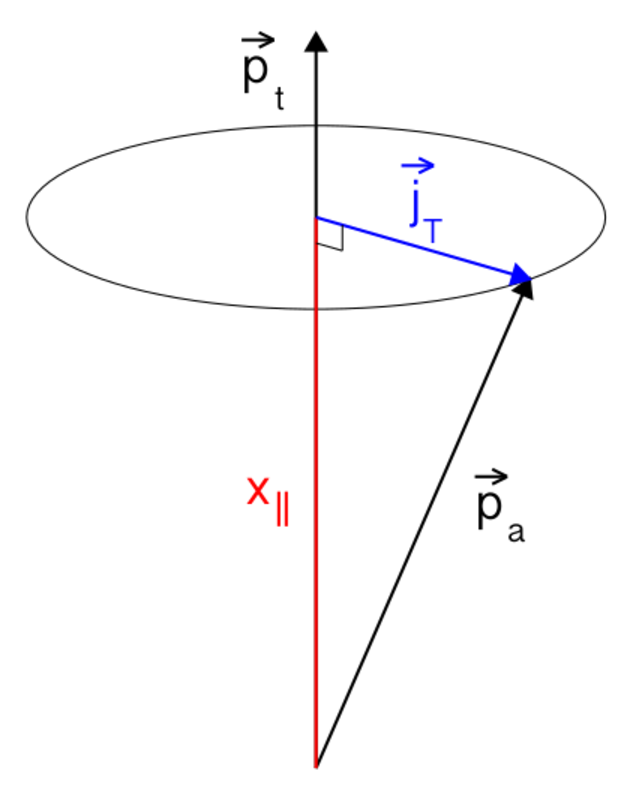
\includegraphics[width = 0.30\textwidth]{figures/jtwithrightangle}
    \end{center}
    \caption{Illustration of $\vjt{}$. The jet fragmentation transverse momentum, $\vjt{}$, is defined as the transverse momentum component of the associated particle momentum, $\vec{p}_{\mathrm{a}}$, with respect to the jet momentum, $\vec{p}_{\mathrm{jet}}$.}
    \label{fig:jtdefinition}
  \end{figure}


The resulting signal distribution are fitted with a 2 component function. Gaussian is used component for low $\jt{}$ and an inverse gamma component for high $\jt{}$. The gaussian is taken to have the center at $\jt{} = 0$. 

$$\frac{1}{N_{\mathrm{jets}}}\frac{\mathrm{d}N}{\jt{} \mathrm{d}\jt{}} = \frac{B_2}{B_1\sqrt{2\pi}}e^{-\frac{\jt{}^2}{2B_1^2}}+\frac{B_3B_5^{B_4}}{\Gamma\left(B_4\right)}\frac{e^{-\frac{B_5}{\jt{}}}}{\jt{}^{B_4+1}}$$

To achieve stable results he fitting is performed in two steps. First each component is fitted separately. Gaussian component is fitted to the low end in $\jt{}$. Fitting the gaussian component to the entire distribution produces the same result. Inverse gamma component is fitted to $\jt{}$ above 1. After getting the results from the individual fits they are combined into a single function with starting values from the individual results and an additional fit is performed.

After getting the fit function we extract $\sqrt{\left<\jt{}^2\right>}$ (RMS) and yield values separately from each component. The narrow component RMS is

$$\sqrt{\left<\jt{}^2\right>}=\sqrt{2}B_1,$$

and the wide component RMS value is calculated as 

$$\sqrt{\left<\jt{}^2\right>}=\frac{B_5}{\sqrt{\left(B_4-2\right)\left(B_4-3\right)}},$$

where it is required that $B_4 > 3$.

%A \textsc{Pythia}~8 simulation was performed to gain support for the separation of these components. To create a clean di-jet event sample, \textsc{Pythia}~8 was initialized to produce two hard gluons with a constant invariant mass for each event. The final-state QCD shower in \textsc{Pythia}~8 is modeled as a timelike shower, as explained in Ref.~\cite{newPythiaShower}. Two simulations were studied, one where the final-state shower was present and one where it was disabled. Without the final-state shower, the hadronization of the leading parton via Lund string fragmentation~\cite{lundString} develops without a QCD showering phase preceding it. When the final-state shower is allowed, the partons go through both showering and hadronization. The results of this study are presented in \fig{fig:componentsFromResonance}. 
%The squares show a nearly Gaussian distribution resulting from the case when the final-state shower is disabled. The circles are obtained when the final-state shower is enabled. A long tail is observed which was not seen in the case with final-state shower off. To estimate the QCD showering component, it is assumed that hadronization dominates at low $\jt{}$, and the distributions from the two simulations coincide at $\jt{} = 0$. This scaling is then applied, since without QCD splittings the partons hadronize at higher scale, producing more particles. With the subtraction of the "hadronization only" -distribution from the total one, the QCD showering part can be separated. This is represented by the diamond symbols in \fig{fig:componentsFromResonance}.
%  
%  \begin{figure}
%    \begin{center}
%      \includegraphics[width = 0.65\textwidth]{figures/pythia_fitComponents_updatedDetails_pTt=6v0-8v0_xe=0v4-0v6}
%    \end{center}
%    \caption{(Color online). Results from a \textsc{Pythia}~8 study with a di-gluon initial state. The circular symbols are obtained when the final-state shower is enabled. The square symbols show the distribution without final-state showering. The diamond symbols representing soft radiation are obtained as a difference between the other two distributions. The distribution without final-state showering is fitted with a Gaussian and the soft radiation part with an inverse gamma function.}
%    \label{fig:componentsFromResonance}
%  \end{figure}  
%  
%This study shows a possible factorization of the showering and hadronization parts of the jet fragmentation in \textsc{Pythia}~8. Based on simulations, template fit functions for hadronization and showering components have been estimated and used to extract the corresponding terms from the data. Since $\vjt{}$ is a two-dimensional vector, using two-dimensional forms for the fit functions allows to extract the final results from the functions more easily. Assuming that there is no dependence on the polar angle of the vector, the angle can be integrated out and the distributions written as a function of the length of the vector. The hadronization part can be described by a Gaussian:
%\begin{equation}
%f_{G}(\jt{}) = \frac{A_{2}}{A_{1}^{2}} \, e^{-\frac{\jt{}^{2}}{2 A_{1}^{2}}},
%\label{eq:gauss}
%\end{equation}
%and the showering part by an inverse gamma function of the form:
%\begin{equation}
%f_{IG}(\jt{}) = \frac{A_{3} \, A_{5}^{A_{4}-1}}{\Gamma(A_{4}-1)} \, \frac{e^{-\frac{A_{5}}{\jt{}}}}{\jt{}^{A_{4}+1}}\;,
%\label{eq:inverseGamma}
%\end{equation}  
%where $A_{1\ldots5}$ are the free fit parameters. In this paper, the hadronization part will be called the narrow component and the showering part the wide component.
%  
%To determine the $\jt{}$ distribution in data, all charged particles inside each $\xlong$ bin are paired with the leading particle and $\jt{}$ is calculated for each of these pairs in an event. In the data, in addition to the signal, a background component mostly due to the underlying event is observed. Examples of measured $\jt{}$ distributions with background included and subtracted are presented in \fig{fig:jtdistribution}. An $\eta$-gap method is used to estimate the background contribution. Pairs with $|\Delta\eta| > 1.0$ are considered as background from the underlying event. The background templates for the analysis are built by randomizing the pseudorapidities for the trigger and the associated particles, following the inclusive charged particle pseudorapidity distributions. Twenty randomized pairs are generated from each background pair to improve the statistics for the background. The template histograms, generated in bins of $\pt{t}$ and $\xlong$, are then fitted to the $\jt{}$ distribution together with a sum of a Gaussian function and an inverse gamma function. It can be seen from \fig{fig:jtdistribution} that the fit is in good agreement with the data, except in the region around $\jt{} \sim 0.4~\GeVc$, where the data shows an increase with respect to the fit function. \textsc{Pythia} studies show that this structure is caused by correlations from neutral meson decays, dominated by decays of $\rho^{0}$ and $\omega$, where one of the decay daughters is the leading charged particle in the event. The effect of this structure is taken into account in the evaluation of the systematic uncertainties.
%
%  \begin{figure}
%    \begin{center}
%      \subfigure{ \includegraphics[width = 0.42\textwidth]{figures/jtdistribution_pp7v0TeV_GlobalSDD_bggausslevy_symbols_LPTrigg_C=0-100_ptt=6-8_xe=0v2-0v4_R=1v0_BG=0}}
%      \subfigure{\includegraphics[width = 0.42\textwidth]{figures/jtsignal_pp7v0TeV_GlobalSDD_bggausslevy_symbols_LPTrigg_C=0-100_ptt=6-8_xe=0v2-0v4_R=1v0_BG=0}}
%    \end{center}
%    \caption{(Color online). \emph{Left:} Measured $\jt{}$ distribution including a three-component fit. The three components describe the background (x-symbols), hadronization (long dashed line), and showering (short dashed line). \emph{Right:} The same $\jt{}$ distribution but with background subtracted.}
%    \label{fig:jtdistribution}
%  \end{figure}
%
%The goal of the analysis is to determine the root-mean-square (RMS) values and yields of the narrow and wide $\jt{}$ components. These are calculated from the parameters of the fit functions in equations~\eqref{eq:gauss} and~\eqref{eq:inverseGamma}.

\section{Systematic uncertainties}
\label{sec:systematicerrors}
The systematic uncertainties in this analysis come from the background estimation, the unfolding procedure and the cuts used to select the tracks. Tracking uncertainties are estimated from variations of the track selection cuts defined in Sec.~\ref{sec:experimentaldetails}. The resulting variations in RMS are shown in Tab. \ref{tab:systematics}. The uncertainties from unfolding and background subtraction are of the same magnitude. 

The systematics in background estimation were studied using an alternative method to extract the background, mainly the random background method. The resulting uncertainty is below 5 \% for the wide component RMS and below 9\% for the narrow component RMS. 

The systematics that arise from the unfolding procedure were estimated by performing the unfolding with two separate methods. The primary method in the analysis was the iterative unfolding method. As a secondary method an SVD unfolding method was performed on the data. In a \textsc{Pythia} closure test the true distribution was in general found to be between the unfolded distributions from the iterative and SVD method. The difference between the methods when unfolding data should give a reasonable estimate of the unfolding uncertainty. The resulting uncertainty is below 8\% for both wide and narrow component RMS.

The different sources of systematic uncertainties were taken as uncorrelated and thus added in quadrature. The resulting uncertainty is 9 \% for the wide component RMS and 12 \% for the narrow component RMS. 

\begin{table}[htb]
\centering
\caption{Summary of systematic errors}
\label{tab:systematics}
\begin{tabular}{ l | c | r }
  Systematic & Wide RMS & Narrow RMS \\
    \hline			
  Background & 5 \% & 9 \% \\
  Unfolding & 8 \% & 8 \% \\
  Tracking & ? \% & ? \% \\
  Total & 9 \% & 12\% \\
  \hline
  \end{tabular}
  \end{table}

There is no tracking and no unfolding uncertainty in the Monte Carlo simulations. 


%
%The systematic uncertainties considered for this analysis arise from the background determination, the signal fitting procedure and the cuts used to select the tracks. The uncertainties related to the tracking are estimated from variations of the track selection cuts defined in Section~\ref{sec:experimentaldetails}. The resulting variations of the RMS and yield are below 3~\% in most cases, but effects up to 17~\% are observed for the yield of the wide component. The tracking efficiency contributes to the uncertainty of the yields only. This uncertainty is estimated from the difference between data and simulation in the TPC-ITS track matching efficiency as is previously done in Refs.~\cite{spectrumReferencePp} and~\cite{spectrumReferencepPb}.  For $\pp$ this uncertainty is 5~\% and for $\pPb$ 4~\%. The effect where the subleading track is reconstructed as a leading track, because of detector inefficiencies, was studied using simulations and found to be negligible due to steep slope of the trigger spectrum.
%
%The main source of uncertainty from the background evaluation comes from the background region definition. As an alternative method to the default procedure, uncorrelated background templates are generated from particles with $R = \sqrt{\Delta\varphi^2 + \Delta\eta^2} > 1$ instead of those at large $\Delta\eta$, and pseudorapidities for the particle pairs are randomized together with azimuthal angles. The associated uncertainty is typically below 5~\%, but for the yield of the wide component the uncertainty can grow up to 46~\% in the lowest $\pt{t}$ and $\xlong$ bins where the signal to background ratio is the worst (0.84 for $\pp$ and 0.33 for $\pPb$). Changing the size of the $\eta$-gap produces small uncertainties compared to other sources, usually below 2~\%. The effect of changing the number of new pairs generated for the background from 20 to 15 or 25 was also checked, but this was found to be negligible and is not included in the total uncertainties.
%
%The dominant source of uncertainty results from decaying neutral mesons. Even though this is a physical correlation in the $\jt{}$ distribution, it cannot be attributed to QCD showering or hadronization. The effect of the decay mesons is estimated from a variation of the fit range, excluding the region where the data shows an increase with respect to the fit function. The excluded region is $0.25 < \jt{} < 0.45\,\GeVc$, $0.2 < \jt{} < 0.6\,\GeVc$ or $0.2 < \jt{} < 0.65\,\GeVc$ for the $\xlong$ bins  $0.2 < \xlong < 0.4$,  $0.4 < \xlong < 0.6$ and  $0.6 < \xlong < 1.0$, respectively. For the yield of the wide component the uncertainty can go up to 60~\% in the $0.4 < \xlong < 0.6$ bin at low $\pt{t}$. In most cases, this uncertainty is well below 10~\%. For the signal fit, the difference between fitting the background and the signal simultaneously and only the signal, after background subtraction, was evaluated. The uncertainty from this source was found to be typically smaller than 3~\%, which is small compared to other sources.
%
%The different sources of systematic uncertainties were considered as uncorrelated and added in quadrature accordingly. In general, the systematic uncertainties for the wide component are larger than for the narrow component, since the signal to background ratio is significantly smaller for the wide component. Also the uncertainties for the yield are larger than for the RMS. The uncertainties are also $\pt{t}$ and $\xlong$ dependent. For different results and datasets, the total systematic uncertainties vary within the ranges summarized in Tab.~\ref{tab:uncertainties}. The smallest uncertainty of $1.6$~\% for the narrow component RMS is found for the $0.2 < \xlong < 0.4$ and highest $\pt{t}$ bins while the largest uncertainty of 73~\% for the yield  of the wide component is found from the $0.4 < \xlong < 0.6$ and lowest $\pt{t}$ bins .
%
%\begin{table}
%  \begin{center}
%    \begin{tabular}{cccc}
%      \toprule
%                                             &       &\multicolumn{2}{c}{Total relative uncertainty} \\
%                                             &       &      $\pp$        &      $\pPb$        \\
%                                             \hline
%        \multirow{ 2}{*}{Narrow component}   &  RMS  &  $1.6 - 6.2\,\%$  &   $1.6 - 8.5\,\%$  \\
%                                             & yield &  $5.2 - 21\,\%$   &   $5.4 - 13\,\%$   \\
%        \multirow{ 2}{*}{Wide component}     &  RMS  &  $1.9 - 7.4\,\%$  &   $3.0 - 14\,\%$   \\
%                                             & yield &  $8.5 - 48\,\%$   &   $13  - 73\,\%$   \\
%        \bottomrule
%    \end{tabular}
%  \end{center}
%  \caption{Total systematic uncertainties for RMS and yield of the narrow and wide components in $\pp$ and $\pPb$ collisions. The ranges reflect $\pt{t}$ and $\xlong$ dependence of the studied observables.}
%  \label{tab:uncertainties}
%\end{table} 
%
%The systematic uncertainty estimation is done also for the \textsc{Pythia} and Herwig simulations, which are compared to the data. As the same analysis method is used for simulations and data, also the same methods to estimate the systematic uncertainty can be applied. For the simulations, the uncertainty is estimated from the background determination and signal fitting. There is no tracking uncertainty in the simulations.

\section{Results}
\label{sec:results}

Distributions of $\jt{}$ after unfolding and background subtraction are shown in Fig. \ref{fig:jtdist}. The yield at low $\jt{}$ stays constant with increasing $p_{T,\mathrm{jet}}$. At high $\jt{}$ the yield increases and the distributions become wider. In part this is due to kinematical limits. Within a fixed cone the maximum $\jt{}$ depends on the track momentum. 

$$j_{T,\mathrm{max}} \approx R \cdot p_{T,track} $$

With increasing jet $\pt{}$ the possible track momenta also increase.

The distributions are fitted using a two component fit. An example of the fitted distribution is shown in Fig. \ref{fig:jtfit}. The $\jt{}$ distributions are well described by the two component model fit. 

\begin{figure}[htb]
\begin{center}
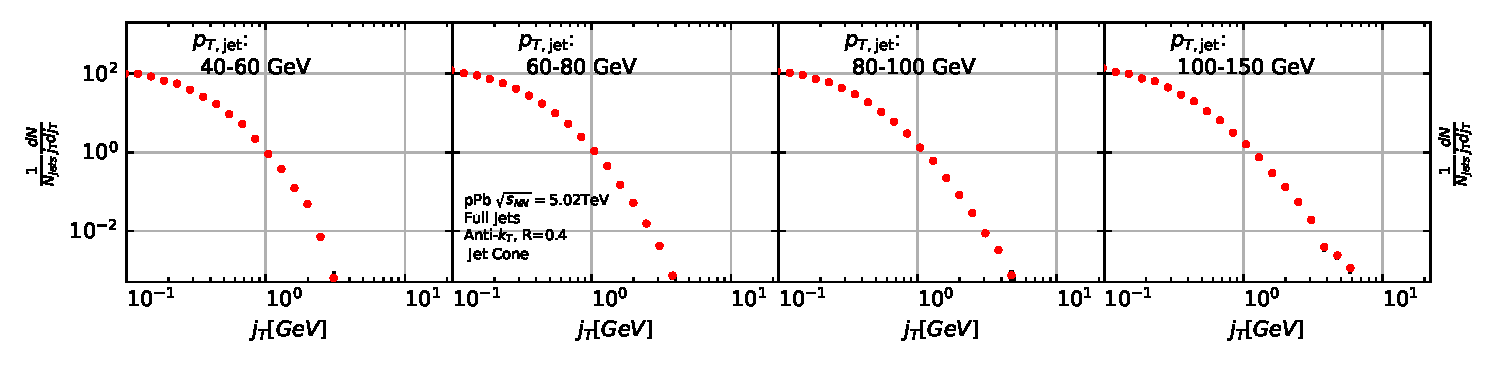
\includegraphics[width=0.95\textwidth]{figures/results/MixedFullJetsR04JetConeJtSignalPtFrom4To8.pdf}
%python Python/DrawSignal.py CF_pPb_legotrain/legotrain_CF_pPb_1839_20180613_LHC13bcde.root 0 4 8
\caption{$\jt{}$ distributions in different jet $\pt{}$ bins.}
\label{fig:jtdist}
\end{center}
\end{figure}

%\begin{figure}[htb]
%\begin{center}
%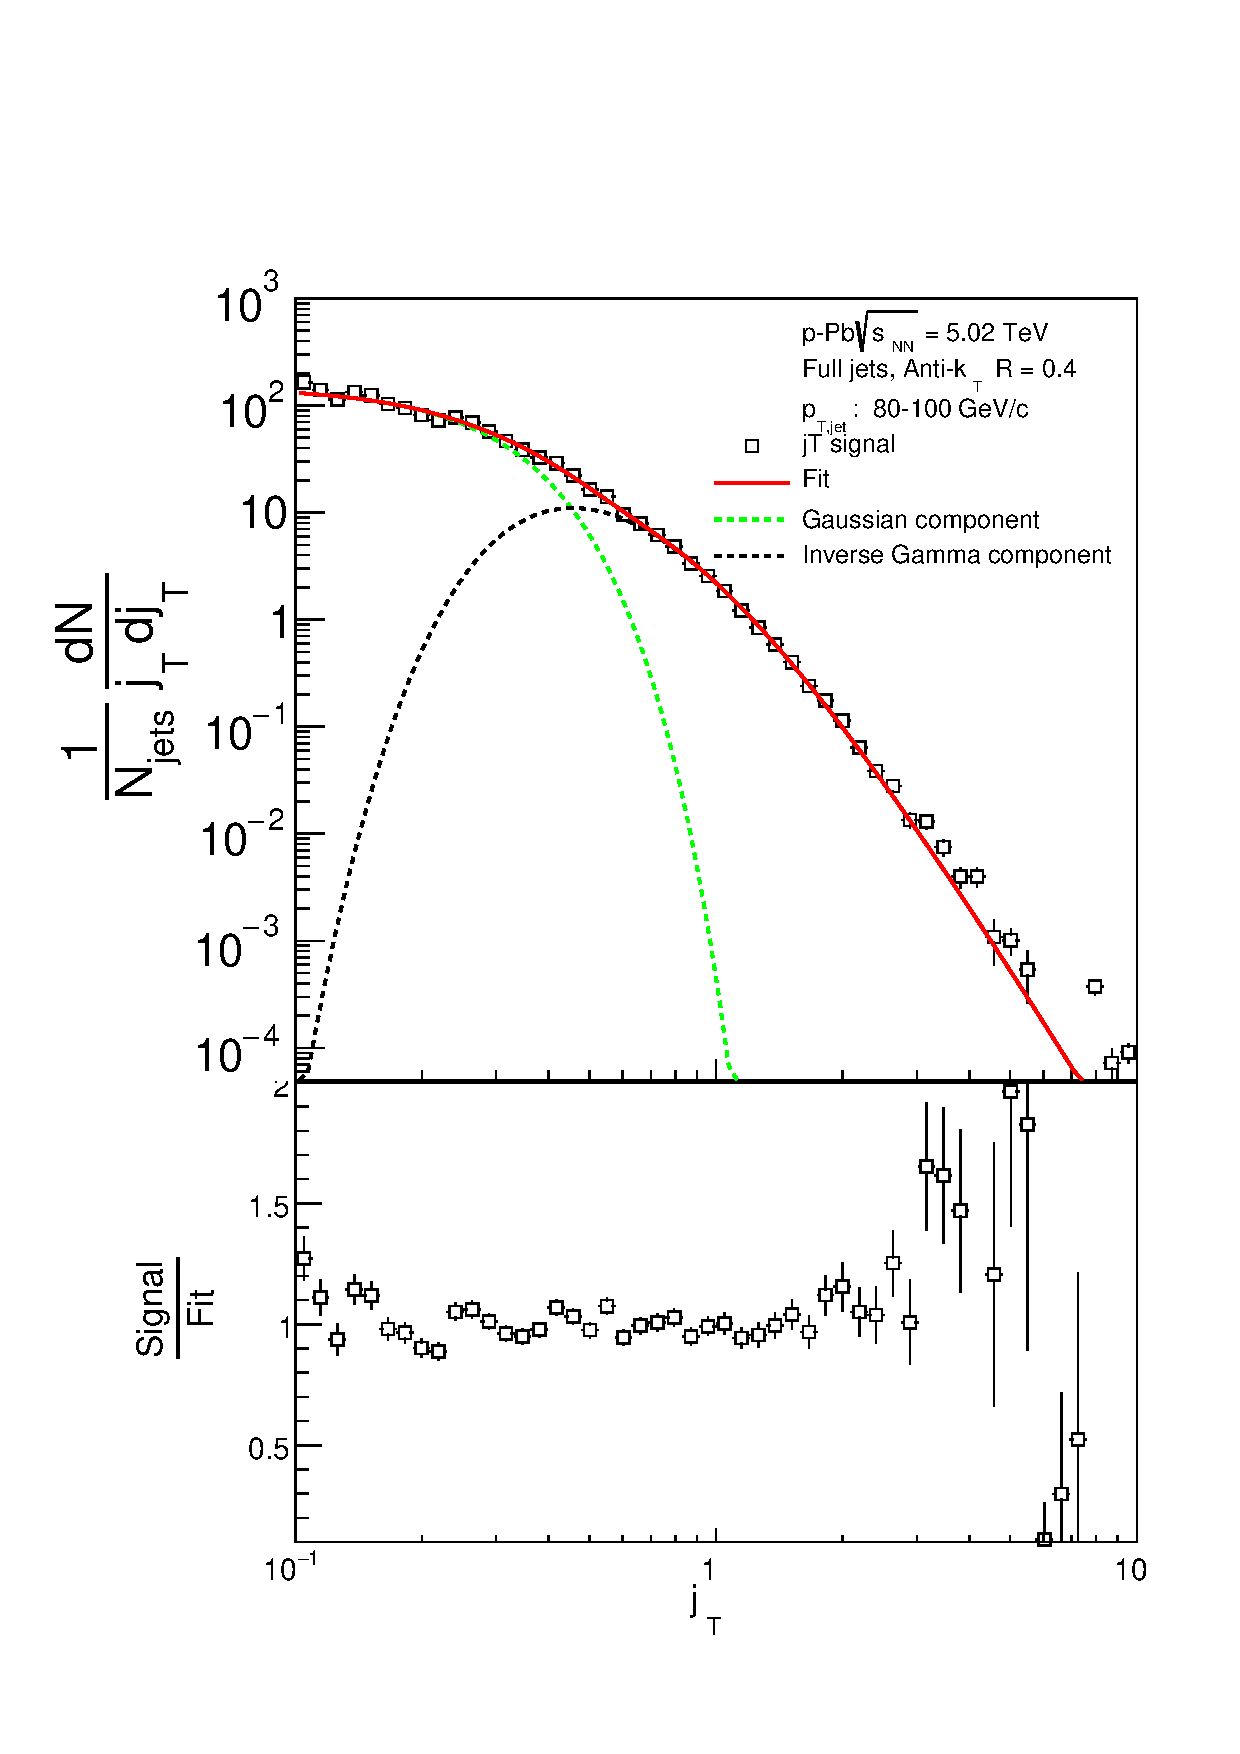
\includegraphics[width=0.5\textwidth]{figures/results/JetConejTSignalFitNFin00JetPt06perconeBgBayes.pdf}
%%python Python/DrawSignal.py CF_pPb_legotrain/legotrain_CF_pPb_1839_20180613_LHC13bcde.root 0 4 8
%\caption{$\jt{}$ distributions in different jet $\pt{}$ bins.}
%\label{fig:jtfit}
%\end{center}
%\end{figure}

The per jet yields and widths of the $\jt{}$ distributions are determined as a function of the transverse momentum of jet. The results are obtained from the area and RMS of the fits to the narrow and wide components of the $\jt{}$ distribution. The RMS $\left(\rms{\jt{}}\,\right)$ values for the narrow component are shown in \fig{fig:rmsgamma} with comparison to Monte Carlo simulations. 

There is clear separation in the width of the wide and narrow components of the $\jt{}$ distributions. The RMS of the wide component is 3-4 times larger than the narrow component RMS. The wide component is assumed to correspond to the fragmentation part of jet formation while the narrow component is linked with the hadronisation phase.

The wide component RMS shows an increasing trend with increasing $p_{T,\mathrm{jet}}$, while the narrow component RMS stays roughly constant. Both of these trends are qualitatively consistent with the results seen in dihadron $\jt{}$ analysis~\cite{ALICEjt}

\textsc{Pythia} describes well the RMS values in both the narrow and wide components. Herwig... \textsc{Pythia} uses the Lund string model for hadronization while Herwig uses a cluster model. It seems ...

%\begin{figure}[htb]
%\begin{center}
%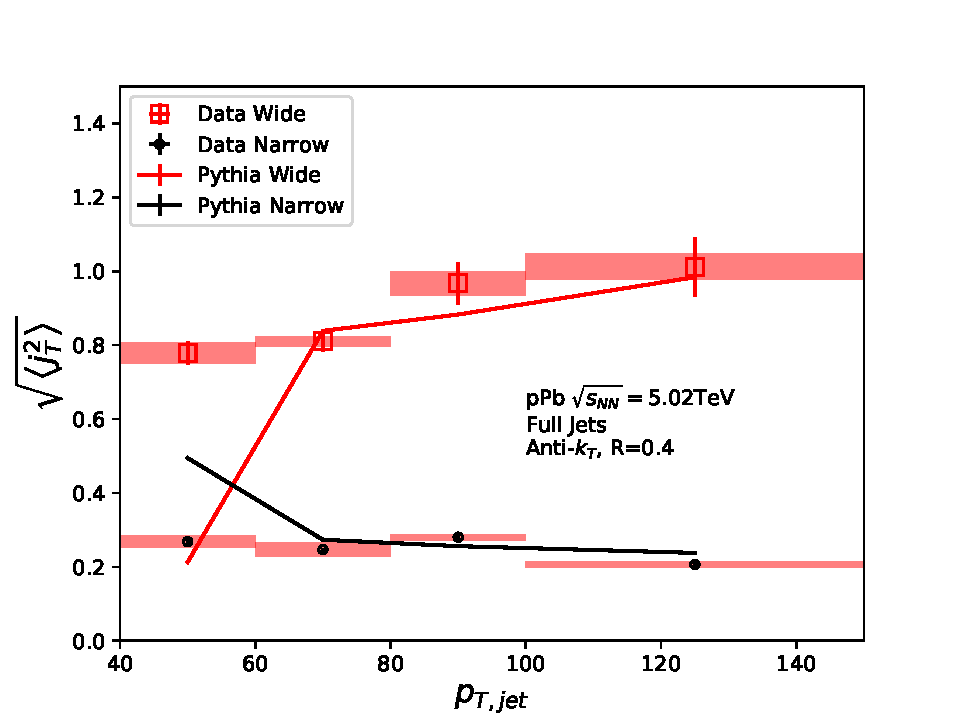
\includegraphics[width=0.55\textwidth]{figures/results/RMSWithSystematics_Pythia}
%\caption{RMS and yield values extracted from the fits for the gaussian (narrow) and inverse gamma (wide) components}
%\label{fig:rmsgamma}
%\end{center}
%\end{figure}

\begin{figure}[htp]
\centering
\subfigure[$\jt{}$ distribution with two component fitting]{\label{fig:jtfit} 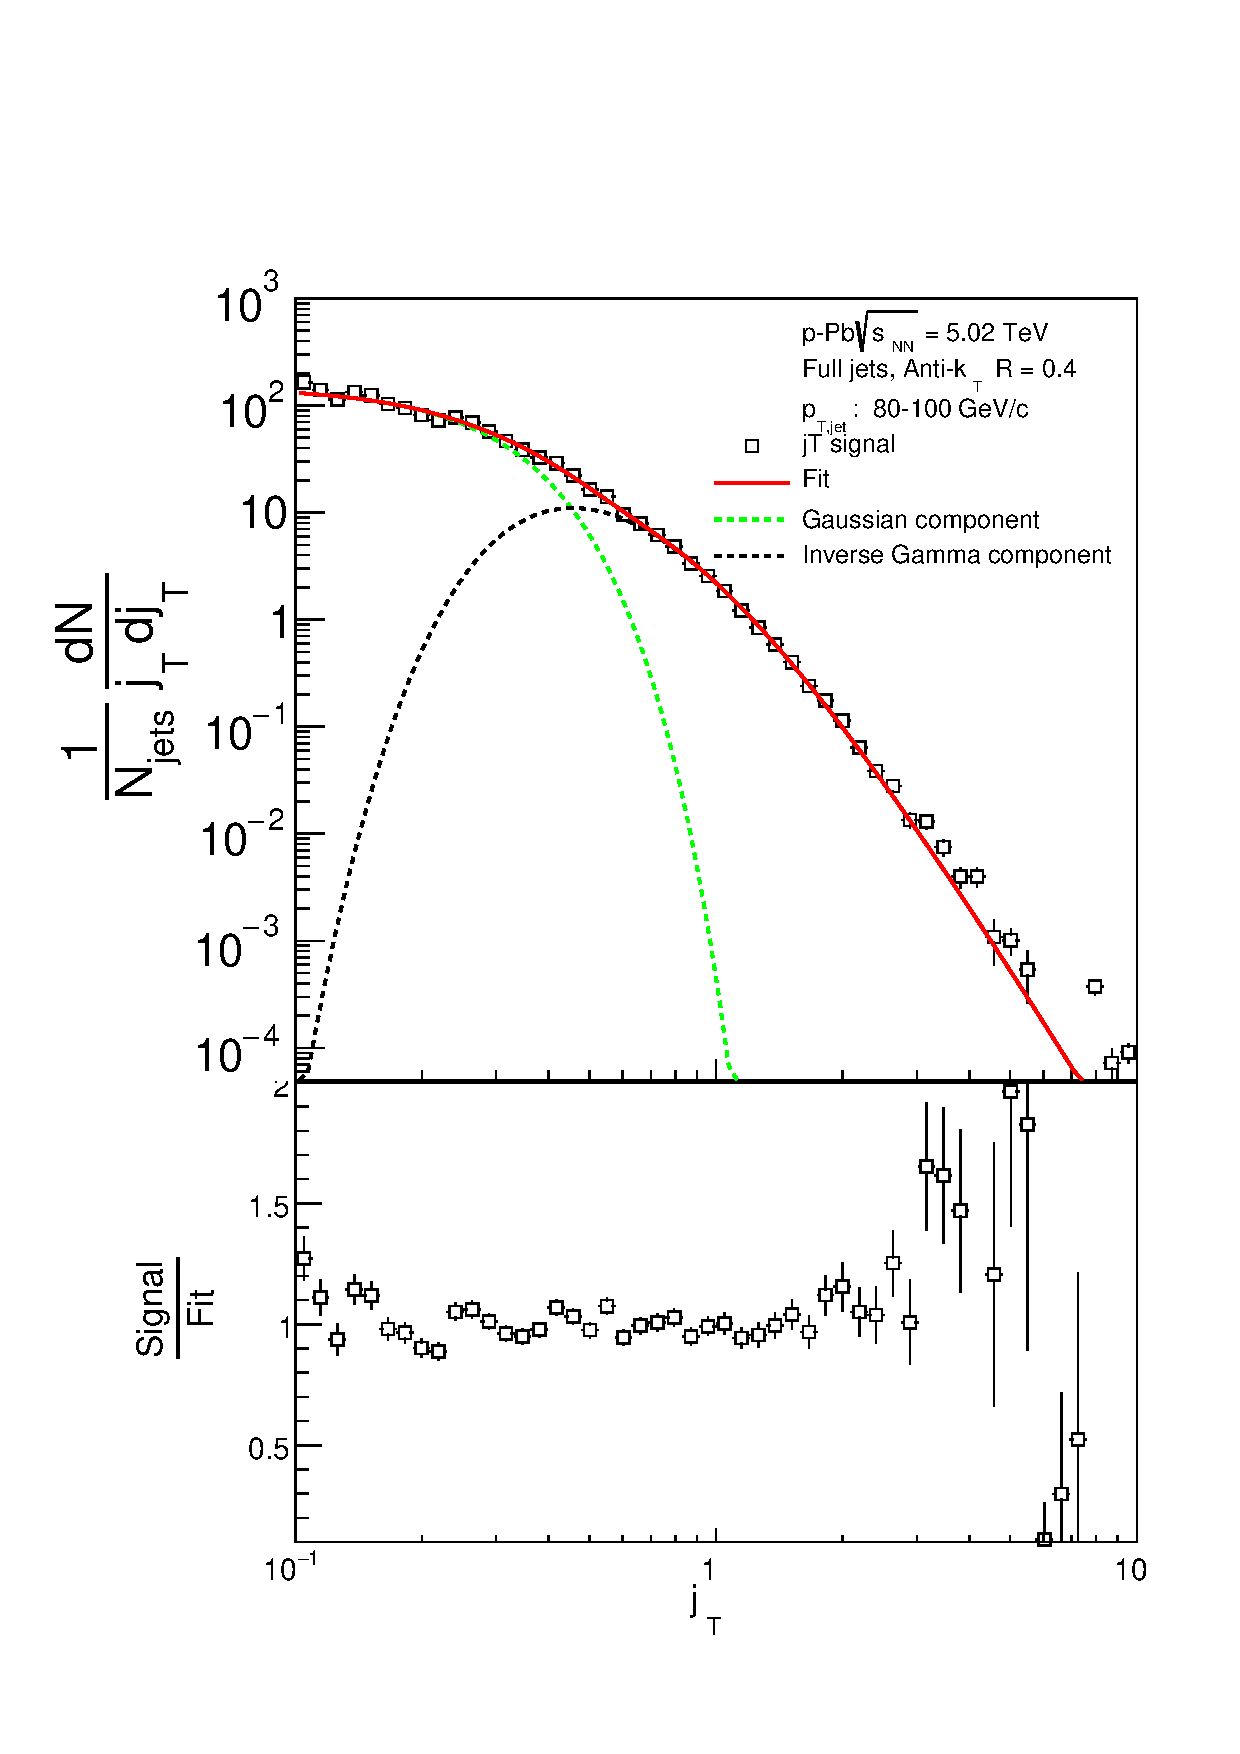
\includegraphics[width = 0.49\textwidth]{figures/results/JetConejTSignalFitNFin00JetPt06perconeBgBayes.pdf}}
\subfigure[RMS and yield values extracted from the fits for the gaussian (narrow) and inverse gamma (wide) components]{\label{fig:rmsgamma} 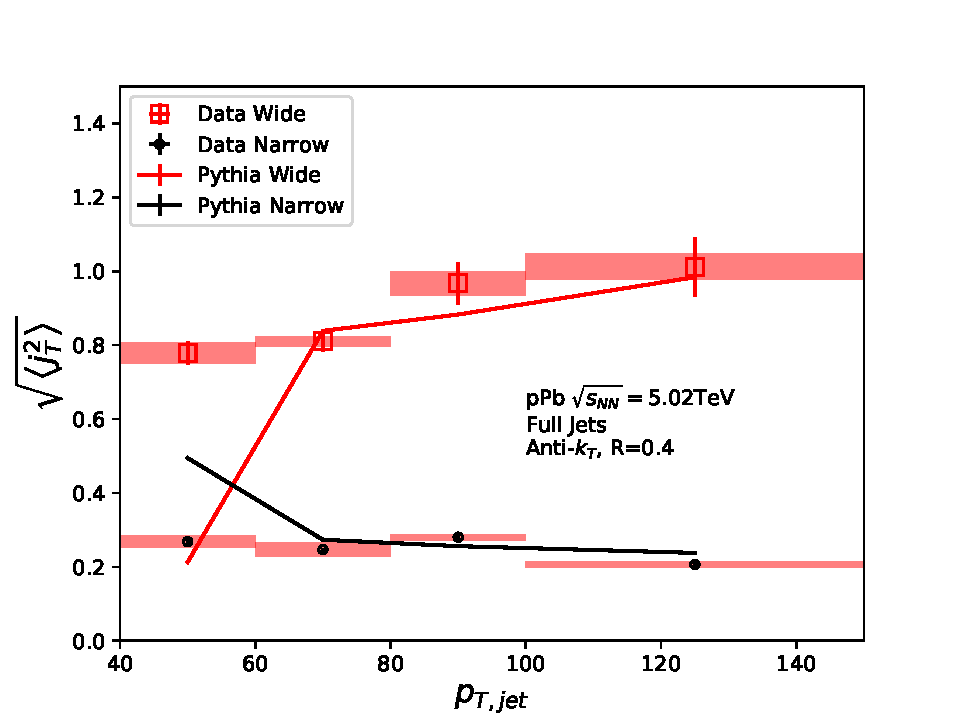
\includegraphics[width = 0.49\textwidth]{figures/results/RMSWithSystematics_Pythia}}
\caption{}
\label{fig:results}
\end{figure}


\FloatBarrier

\subsection{Discussion}
\begin{figure}[htb]
\centering
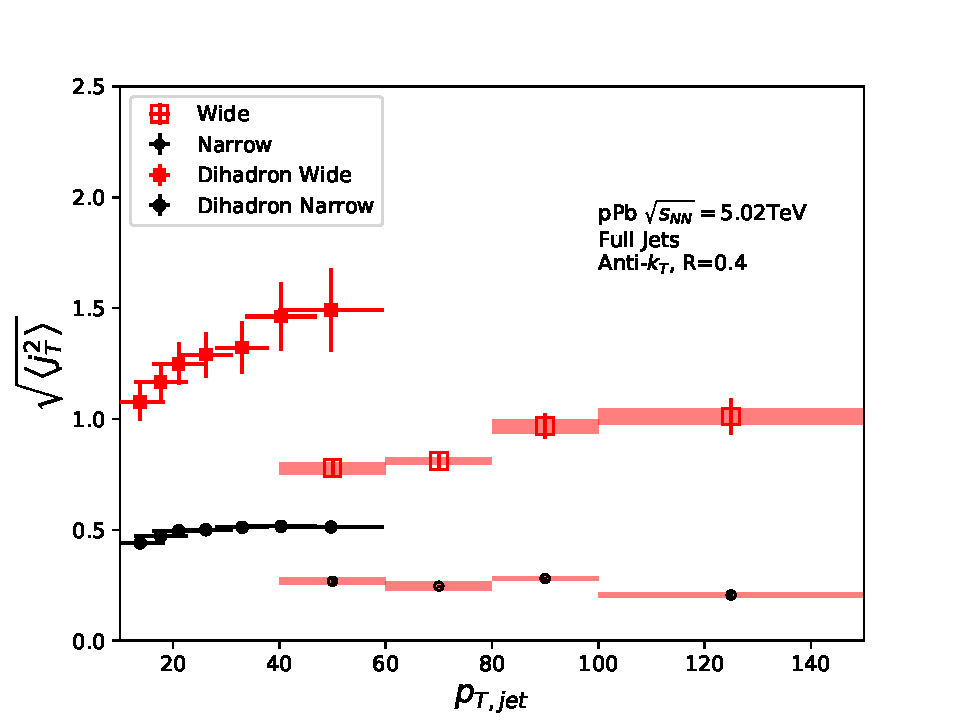
\includegraphics[width=0.55\textwidth]{figures/results/RMSWithSystematics_DihadronJetPt}
%\subfigure{ 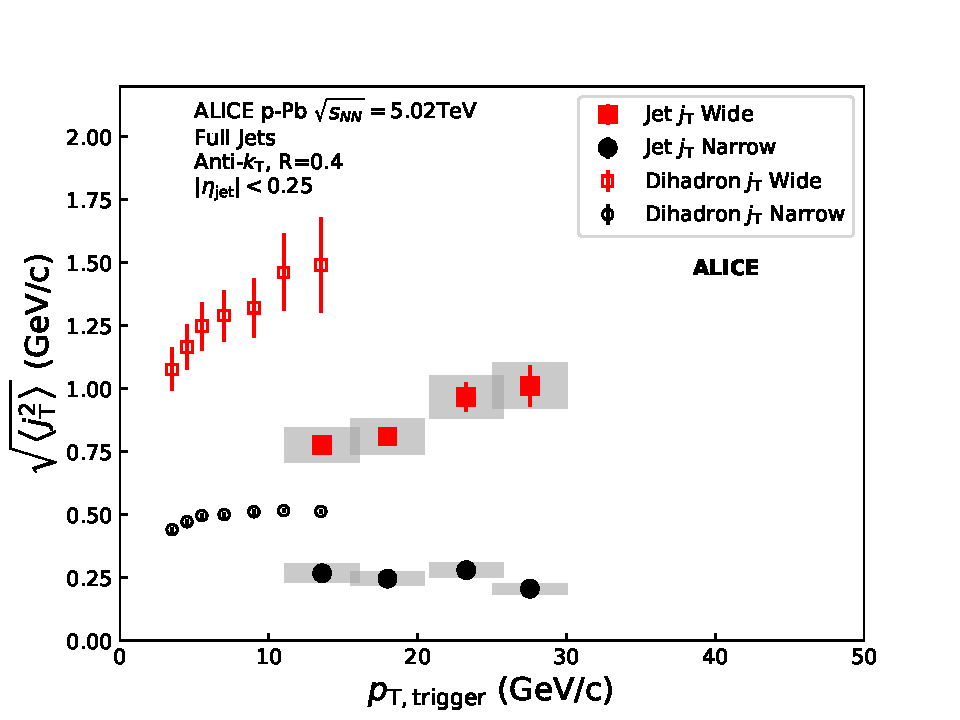
\includegraphics[width = 0.42\textwidth]{figures/results/RMSWithSystematics_DihadronTriggerPt}}
%\subfigure{ 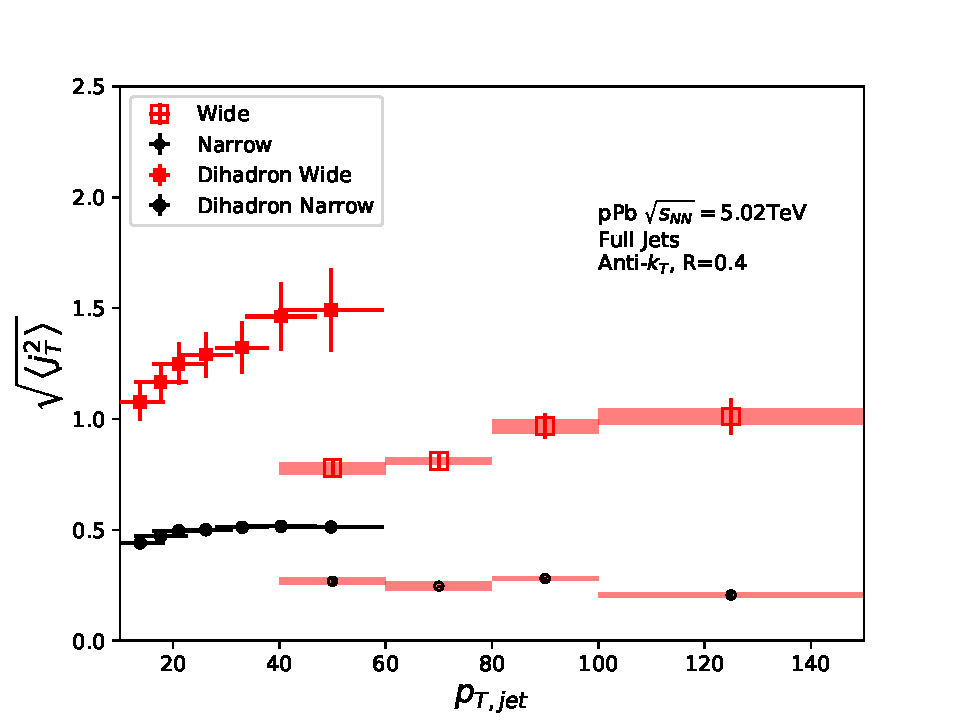
\includegraphics[width = 0.42\textwidth]{figures/results/RMSWithSystematics_DihadronJetPt}}
\caption{Comparison of results with dihadron $\jt{}$ results. Dihadron trigger $\pt{}$ bins are converted to jet $\pt{}$  bins  using observed mean  $p_{T,\mathrm{jet}}$ values in $p_{T,\mathrm{trigger}}$ bins. Dihadron results are for $0.2 < x_{||} < 0.4$ }
\label{fig:DihadronComparison}
\end{figure}

Comparison to $\jt{}$ results from dihadron analysis ~\cite{ALICEjt} is shown in Fig. \ref{fig:DihadronComparison}. Trigger $\pt{}$ bins used in dihadron analysis are converted to jet $\pt{}$ bins using observed average jet $\pt{}$ values in leading track momentum bins. Simlarly jet $\pt{}$ bins are converted to $p_{T,\mathrm{trigger}}$ bins using average leading track $\pt{}$ values in $p_{T,\mathrm{jet}}$ bins.

The trends are similar in dihadron and jet $\jt{}$ results. Wide component RMS values tend to increase with increasing $p_{T,\mathrm{trigger}}$/$p_{T,\mathrm{jet}}$. Narrow component RMS increases slightly in dihadron analysis but not in jet $\jt{}$, WHY? (Depends on $x_{||}$ bin in dihadron)

In general dihadron $\jt{}$ gives wider distributions with larger RMS values. In jet analysis the cone size limits width and thus the RMS values. With increasing cone size one gets increasing wide RMS values as seen in Fig. \ref{fig:Rcomparison}. This should be the dominant factor.

\begin{figure}[htp]
\centering
\subfigure{ 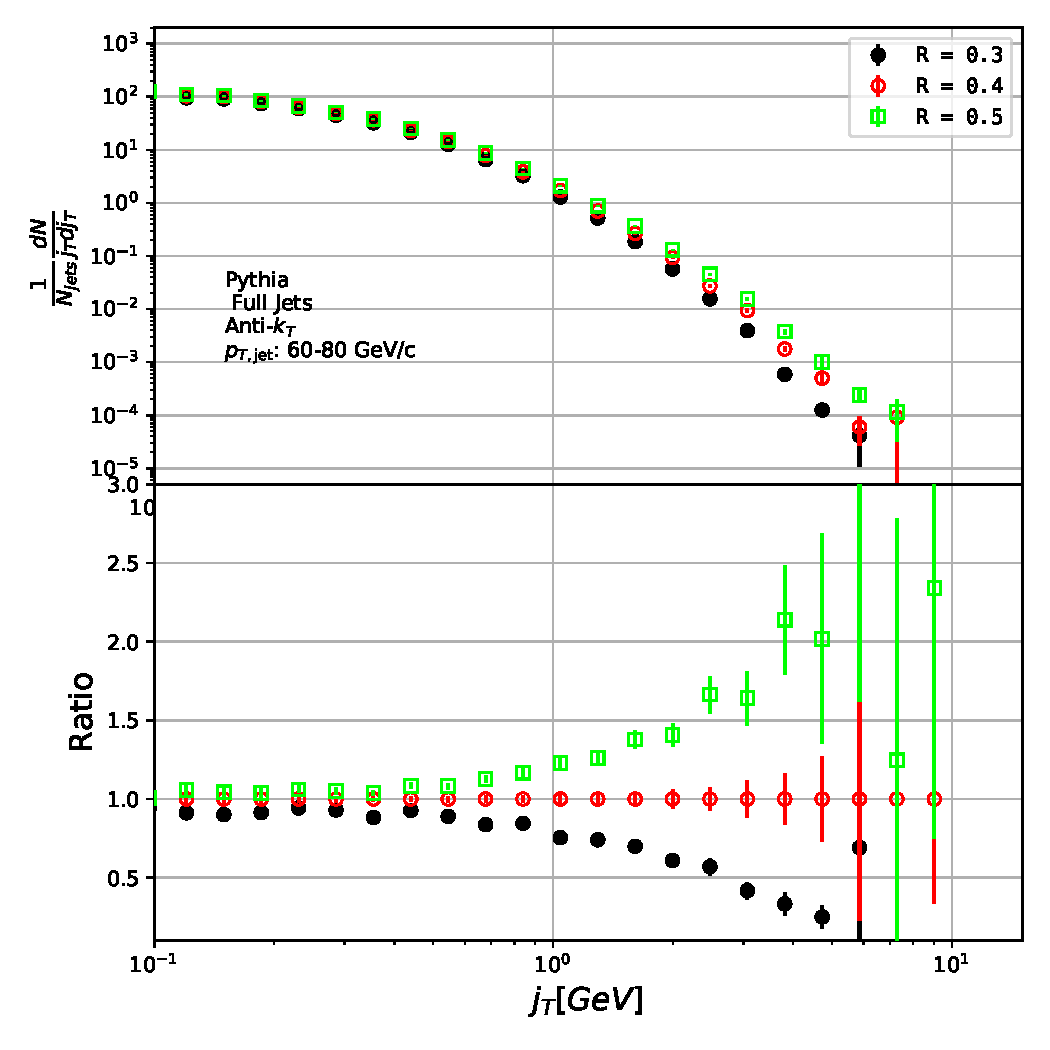
\includegraphics[width = 0.4\textwidth]{figures/results/RcomparisonSignalPt6080.pdf}}
\subfigure{ 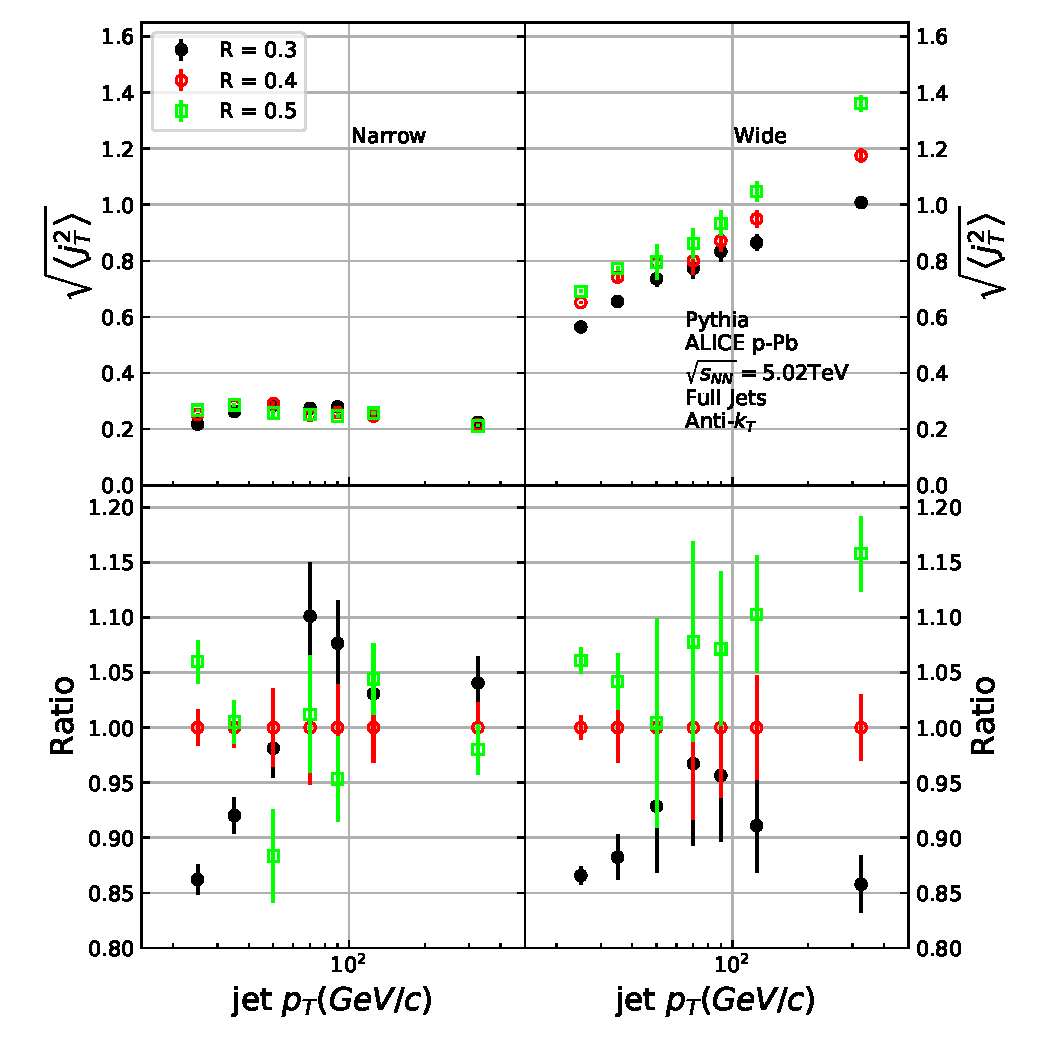
\includegraphics[width = 0.4\textwidth]{figures/results/RcomparisonRMS.pdf}}
\caption[\textsc{Pythia} $R$ parameters $\jt{}$]{Effect of changing $R$ parameter in jet finding on $\jt{}$ distributions}
\label{fig:Rcomparison}
\end{figure}


Effect of the $R$ parameter choice is studied in \textsc{Pythia}. Having a fixed cone puts hard limits on the possible $\jt{}$ values. Increasing the cone size loosens these limits and allows higher $\jt{}$ values. The results are shown in Fig. \ref{fig:Rcomparison}. Left hand side shows the $\jt{}$ distributions. There is very little change in low $\jt{}$ but at high $\jt{}$ the yield increases. 

This is also seen in the RMS values shown in the right hand side of Fig. \ref{fig:Rcomparison}, where the change in wide component RMS is about 10\% when going from $R=0.4$ to $R=0.3$ or $R=0.5$. With the narrow component values the situation is less clear. At low jet $\pt{}$ larger $R$ parameter leads to larger RMS values, but at hight $p_{T,\mathrm{jet}}$ the situation is reversed; increasing the $R$ parameter decreases RMS values.

Additionally the leading track is an imperfect estimate of the jet/original parton. Because the leading track in general is at an angle compared to the jet axis, the resulting $\jt{}$ values are different. In practice the jet axis found by the jet finding algrorithm tends to minimize the average $\jt{}$ of jet constituents. Thus the yield at high $\jt{}$ is limited and the RMS values are smaller.

A \textsc{Pythia} study was performed where $\jt{}$ was calculated with respect to the leading track momentum, instead of the jet axis. The results are shown in Fig. \ref{fig:RefComparison}. The resulting $\jt{}$ distributions are significantly wider than $\jt{}$ distributions from the typical method. The effect seems to be larger than the effect seen in comparing different $R$ values.

\begin{figure}[htp]
\centering
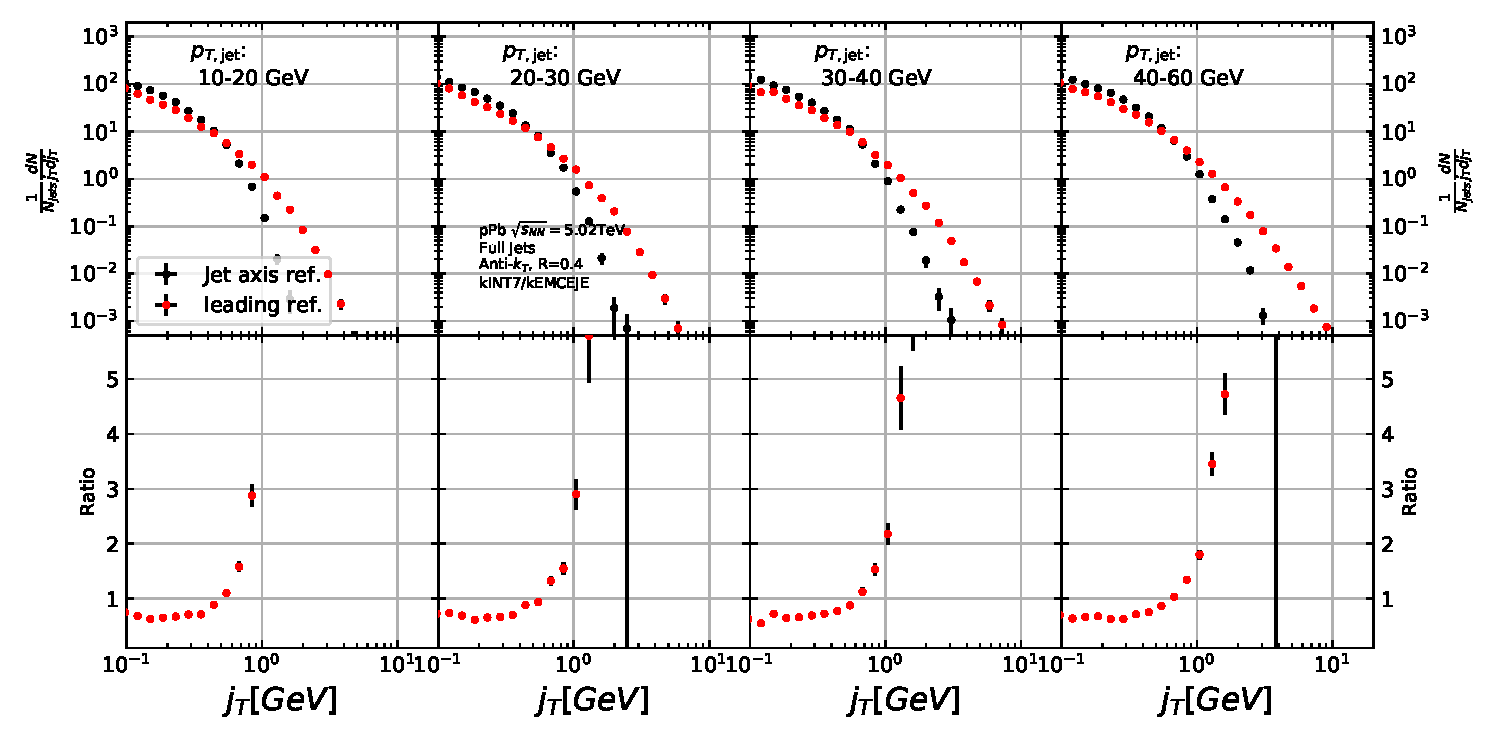
\includegraphics[width=0.55\textwidth]{figures/results/JetVsLeadingRefConst.pdf}
\caption{Results of calculating $\jt{}$ with respect to the jet axis or the leading hadron. The assumption is that because the leading hadron is an imperfect estimate of the jet axis, low $\jt{}$ tracks should on average be shifted to higher $\jt{}$}
\label{fig:RefComparison}
\end{figure}

\section{Conclusions}
\label{sec:conclusions}
In this work two distinct $\jt{}$ components were extracted for narrow and wide contributions using jet reconstruction. RMS values for both components were obtained. The width of the wide component is found to increase for increasing $\pt{jet}$. This is in part explained by the changing kinematical limits when going to higher $\pt{jet}$ which allows higher $\pt{track}$. Additionally the larger phase space allows stronger parton splitting. The results are qualitatively compatible with previous studies that studied $\jt{}$ using two-particle correlations.



%A new method to extract two distinct $\jt{}$ components for  a narrow (hadronization) and wide (QCD branching) contribution using two-particle correlations was presented in this work.  The RMS and per trigger yield were obtained for both components. The width of the narrow component shows only a weak dependence on the trigger particle transverse momentum and no difference between $\pp$ and $\pPb$ collisions. The results from this analysis are also qualitatively compatible with the previous ones at lower $\sqrt{s}$, measured by the PHENIX and the CCOR experiments. All of these observations support the universal hadronization expectation. The width of the wide component is found to increase for increasing $\pt{t}$ in all $\xlong$ bins. This can be explained by stronger parton splitting, which is allowed by a larger phase space. A similar argument can be used to explain why the wide component has not been previously observed at the ISR or at RHIC since the larger collision energy at the LHC increases phase space for QCD splittings. As there is no difference in the wide component RMS between $\pp$ and $\pPb$, cold nuclear matter effects do not play a large role in this kinematic regime. \textsc{Pythia}~8 and Herwig~7 simulations describe the widths for both components well, but both simulations overestimate the yield of the narrow component. These measurements could be used to further constrain the parameters in the models to better reproduce the data.
%
%An interesting follow-up study would be to look at the same measurement in heavy-ion collisions. As it is shown that there are no cold nuclear matter effects in $\pPb$ $\jt{}$ distributions, any modifications in the distributions could be attributed to final-state effects, such as partonic energy loss in the quark-gluon plasma. The wide component might be able to discriminate between different jet shape modification mechanisms in $\PbPb$ collisions, like interactions with the plasma~\cite{jetBroadeningAA}, color decoherence effects~\cite{antiangularOrdering}, and changes in relative quark and gluon jet fractions~\cite{jetShapeQGP}.
